\documentclass[fleqn,10pt]{olplainarticle}
% Use option lineno for line numbers 

\usepackage[nolist]{acronym}

\usepackage{ifdraft}


%% JAKOB commands:
\newcommand{\Jakob}[1]{
    \ifoptionfinal{}{\color{orange}{\itshape{#1}}\color{black}}
    }{\ignorespaces}
    
%% quotes at the beginning of chapters: chapterQuote
\newcommand{\chapterQuote}[2]{
    \begin{center}
    \textit{#1}  
    \end{center}
    \begin{flushright}
    {#2}
    \end{flushright}
}


%% fonts:
\usepackage{palatino}
\usepackage{euler}

\usepackage{natbib}

\usepackage[obeyFinal]{todonotes}

\usepackage{wrapfig}
\usepackage{multicol}
\usepackage{showlabels}
\usepackage{tabularx}


% to not have longer spaces after periods (end of sentence)
\frenchspacing

% %%%%%%%%%%%%%%%%%%%%%%%%%%%%%%%%%%%%%%%%%%%%%
% Acronyms Patch
%
% Extend acronym package with first letter caps
% https://tex.stackexchange.com/a/150798/117727
% %%%%%%%%%%%%%%%%%%%%%%%%%%%%%%%%%%%%%%%%%%%%%

\makeatletter
\newif\ifAC@uppercase@first%
\def\Aclp#1{\AC@uppercase@firsttrue\aclp{#1}\AC@uppercase@firstfalse}%
\def\AC@aclp#1{%
    \ifcsname fn@#1@PL\endcsname%
        \ifAC@uppercase@first%
            \expandafter\expandafter\expandafter\MakeUppercase\csname fn@#1@PL\endcsname%
        \else%
            \csname fn@#1@PL\endcsname%
        \fi%
    \else%
        \AC@acl{#1}s%
    \fi%
}%
\def\Acp#1{\AC@uppercase@firsttrue\acp{#1}\AC@uppercase@firstfalse}%
\def\AC@acp#1{%
    \ifcsname fn@#1@PL\endcsname%
        \ifAC@uppercase@first%
            \expandafter\expandafter\expandafter\MakeUppercase\csname fn@#1@PL\endcsname%
        \else%
            \csname fn@#1@PL\endcsname%
        \fi%
    \else%
        \AC@ac{#1}s%
    \fi%
}%
\def\Acfp#1{\AC@uppercase@firsttrue\acfp{#1}\AC@uppercase@firstfalse}%
\def\AC@acfp#1{%
    \ifcsname fn@#1@PL\endcsname%
        \ifAC@uppercase@first%
            \expandafter\expandafter\expandafter\MakeUppercase\csname fn@#1@PL\endcsname%
        \else%
            \csname fn@#1@PL\endcsname%
        \fi%
    \else%
        \AC@acf{#1}s%
    \fi%
}%
\def\Acsp#1{\AC@uppercase@firsttrue\acsp{#1}\AC@uppercase@firstfalse}%
\def\AC@acsp#1{%
    \ifcsname fn@#1@PL\endcsname%
        \ifAC@uppercase@first%
            \expandafter\expandafter\expandafter\MakeUppercase\csname fn@#1@PL\endcsname%
        \else%
            \csname fn@#1@PL\endcsname%
        \fi%
    \else%
        \AC@acs{#1}s%
    \fi%
}%
\edef\AC@uppercase@write{\string\ifAC@uppercase@first\string\expandafter\string\MakeUppercase\string\fi\space}%
\def\AC@acrodef#1[#2]#3{%
    \@bsphack%
    \protected@write\@auxout{}{%
        \string\newacro{#1}[#2]{\AC@uppercase@write #3}%
    }\@esphack%
}%
\def\Acl#1{\AC@uppercase@firsttrue\acl{#1}\AC@uppercase@firstfalse}%
\def\Acf#1{\AC@uppercase@firsttrue\acf{#1}\AC@uppercase@firstfalse}%
\def\Ac#1{\AC@uppercase@firsttrue\ac{#1}\AC@uppercase@firstfalse}%
\def\Acs#1{\AC@uppercase@firsttrue\acs{#1}\AC@uppercase@firstfalse}%
% \robustify\Aclp%
% \robustify\Acfp%
% \robustify\Acp%
% \robustify\Acsp%
% \robustify\Acl%
% \robustify\Acf%
% \robustify\Ac%
% \robustify\Acs%

\def\AC@@acro#1[#2]#3{%
    \ifAC@nolist%
    \else%
        \ifAC@printonlyused%
            \expandafter\ifx\csname acused@#1\endcsname\AC@used%
                \item[\protect\AC@hypertarget{#1}{\acsfont{#2}}] #3%
                \ifAC@withpage%
                    \expandafter\ifx\csname r@acro:#1\endcsname\relax%
                        \PackageInfo{acronym}{Acronym #1 used in text but not spelled out in full in text}%
                    \else%
                        \dotfill\pageref{acro:#1}%
                    \fi\\%
                \fi%
            \fi%
        \else%
            \item[\protect\AC@hypertarget{#1}{\acsfont{#2}}] #3%
        \fi%
    \fi%
    \begingroup%
        \def\acroextra##1{}%
        \@bsphack%
        \protected@write\@auxout{}%
            {\string\newacro{#1}[\string\AC@hyperlink{#1}{#2}]{\AC@uppercase@write #3}}%
        \@esphack%
    \endgroup%
}
\makeatother


\begin{acronym} % Give the longest label here so that the list is nicely aligned
\acro{2D}{two-dimensional}
\acro{3D}{three-dimensional}
\acro{AI}{artificial intelligence}
\acro{AM}{additive manufacturing}
\acro{API}{application programming interface}
\acro{AR}{action research}
\acro{asm}{assembly}
    \acroplural{asm}[asm]{assemblies}
\acro{C}{constraint}
\acro{Cf}{functional constraint}
\acro{Cm}{manufacturing constraint}
\acro{CCA}{contact and channel approach}
\acro{CE}{concurrent engineering}
\acro{CAD}{computer aided design}
\acro{CAE}{computer aided engineering}
\acro{CAM}{computer aided manufacturing}
\acro{CAx}{computer aided technologies}
\acro{CC}{configurable component}
\acro{DA}{design automation}
\acro{DEE}{design and engineering engine}
\acro{DfM}{design for manufacturing}
\acro{DfAM}{design for additive manufacturing}
\acro{DMLS}{direct metal laser sintering}
\acro{DP}{design parameter}
\acro{DR}{design rationale}
\acro{DRM}{design research methodology}
\acro{DS}{design solution}
\acro{DS1}{descriptive study one}
\acro{DS2}{descriptive study two}
\acro{DSE}{design space exploration}
\acro{EDR}{engineering design research}
\acro{EF-M}{enhanced function-means}
\acro{EoL}{end of life}
\acro{EWB}{engineering work bench}
\acro{FBO}{fan-blade out}
\acro{FBS}{function-behaviour-structure}
\acro{FCB}{front centre body}
\acro{FEM}{finite element method}
\acro{FF}{fan frame}
\acro{FGOM}{function-geometry object model}
\acro{FM}{function modelling}
\acro{FR}{functional requirement}
\acro{GUI}{graphical user interface}
\acro{HLP}{high-level primitives}
\acro{icb}{is constrained by}
\acro{isb}{is solved by}
\acro{IP}{intellectual property}
\acro{ipmb}{is partially met by}
\acro{iw}{interacts with}
\acro{KBE}{knowledge-based engineering}
\acro{MBSE}{model-based systems engineering}
\acro{MDA}{multi-disciplinary analysis}
\acro{MDO}{multi-disciplinary optimisation}
\acro{MEPHISTO}{Modelling in Early Phases to Investigate System and Technology Options}
\acro{MOKA}{methodology for knowledge based engineering applications}
\acro{NatS}{natural sciences}
\acro{NX}{Siemens NX\textregistered}
\acro{OGV}{outlet guide vane}
\acro{OMFG}{object model for function and geometry}
\acro{omfgDSE}{object model for function and geometry based design space exploration}
\acro{OO}{object-oriented}
\acro{OOP}{object-oriented programming}
\acro{PDM}{product data management}
\acro{PDP}{product development process}
\acro{PD}{product development}
\acro{PLM}{product life-cycle management}
\acro{prt}{part}
    \acroplural{prt}[prt]{parts}
\acro{PS}{prescriptive study}
\acro{rf}{requires function}
\acro{RQ}{research question}
\acro{SAR}[SoAR]{spiral of applied research}
\acro{SE}{systems engineering}
\acro{SED}{Systems Engineering Design}
\acro{SBCE}{set-based concurrent engineering}
\acro{SysML}{systems modelling language}
\acro{TRS}{turbine rear structure}
\acro{UDF}{user defined feature}
\acro{UX}{user experience}
\acro{UML}{unified modelling language}
\end{acronym}

\title{Design Space Exploration of a turbojet part using a combined object model for function and geometry }

\author[1]{Jakob R. Müller}
\author[2]{Second Author}
\affil[1]{jakob.muller@chalmers.se}
\affil[2]{Address of second author}

\keywords{Product development process, Design space exploration, Function modelling, CAD, Aerospace}

\begin{abstract}
Product development, especially in the aerospace industry, hinges on the use of CAD models and the subsequent geometry-based analyses for evaluation of the quality of a concept.
However, the generation (and even variation) of a CAD model to include radical or novel design solutions is an expensive modelling effort.
Furthermore, the focus on CAD models limits the interaction of the developers with the concept of "product function", thereby further reducing the scope of the explored design variants.

To alleviate this, a combined \ac{OMFG} is used in the conceptual development phase of the development of a part for a turbofan engine developed at an aerospace manufacturer.
The approach is tested in the form of a prototype tool through workshops and interviews with practitioners.

Initially the use of the approach provided a certain difficulty for the practitioners through the level of abstraction of the term "function" and the related function modelling approach.
However, once the initially steep learning curve for the modelling approach had been conquered, the practitioners used the approach to explore novel solutions and configurations and appreciated the approach as a good way to quickly generate and evaluate novel concepts.

Although further development in terms of interface design and CAD integration are necessary to evolve the approach out of its prototype stage, it showed a valuable contribution to design space exploration by illustration the design rationale of the product, providing a structured way to capture and integrate novel solutions as well as a clear connection between the abstract functional and the concrete geometrical domain.


\end{abstract}

\begin{document}

\flushbottom
\maketitle
\thispagestyle{empty}

\section{Introduction}
Product development is the realisation of a function in a geometry \citep{Roozenburg1995}.
However, function is hardly represented in the models used in product development.
This leads to an under-explored design space, and product developers potentially missing better performing concepts \citep{Isaksson2016}.



\section{Research approach}
This publication reports from a study in cooperation with an aerospace manufacturer.
The research was performed in an action research approach, where the researchers accompanied the development process investigating into new opportunities for a fan frame \ac{OGV}.

The current state of working was investigated through interviews and observations of the practitioners.
In a workshop for the entire \ac{OGV} development team, a functional decomposition of the part was performed and captured.
Based on this, the researchers created a model in \ac{omfgDSE} for the legacy design.
The design space was then further explored through an online\footnote{The workshop was performed online due to the social distancing regulations caused by the COVID-19 pandemic.} workshop for the \ac{OGV} development team. 
The results were captured in video and through a change protocol in database of the \ac{omfgDSE} tool.

The findings from the workshop were verified through semi-structured in-depth interviews with selected participants of the workshop. \Jakob{these are still outstanding - hopefully after summer!} 

Since the product being in development at the case company, it underlies certain \ac{IP} and export restrictions. 
Therefore, in this publication, a simplified model is used for presentation purposes in order to protect the case company's and their customers' \ac{IP}.
However, the simplified \ac{OGV} model has been verified with the practitioners in order to be able to convey the main functions and solutions of a generic \ac{OGV}.

\section{Results}

\subsection{The omfgDSE approach}
\Jakob{presentation of the approach; EF-M model; CAD coupling; instantiation - more or less a short rundown from CADandA}


\subsection{Case study}
\Jakob{framework and product}
The case study was performed in collaboration with a Swedish aerospace manufacturer. 
The company currently develops a new \ac{FF} \ac{OGV} for future aircraft engines.
The part is located in the bypass of the turbofan engine, positioned just behind the fan, as shown in Figure \ref{fig:ogvInTurbine}.
The set of all \ac{OGV} has the main function to deswirl the airflow from the main rotor, thereby reducing aerodynamic losses.
Furthermore, the vane has a structural function in that it connects the shroud of the bypass to the \ac{FCB}, thereby creating a load path for the turbine mass to the pylon.

\begin{figure}
    \centering
    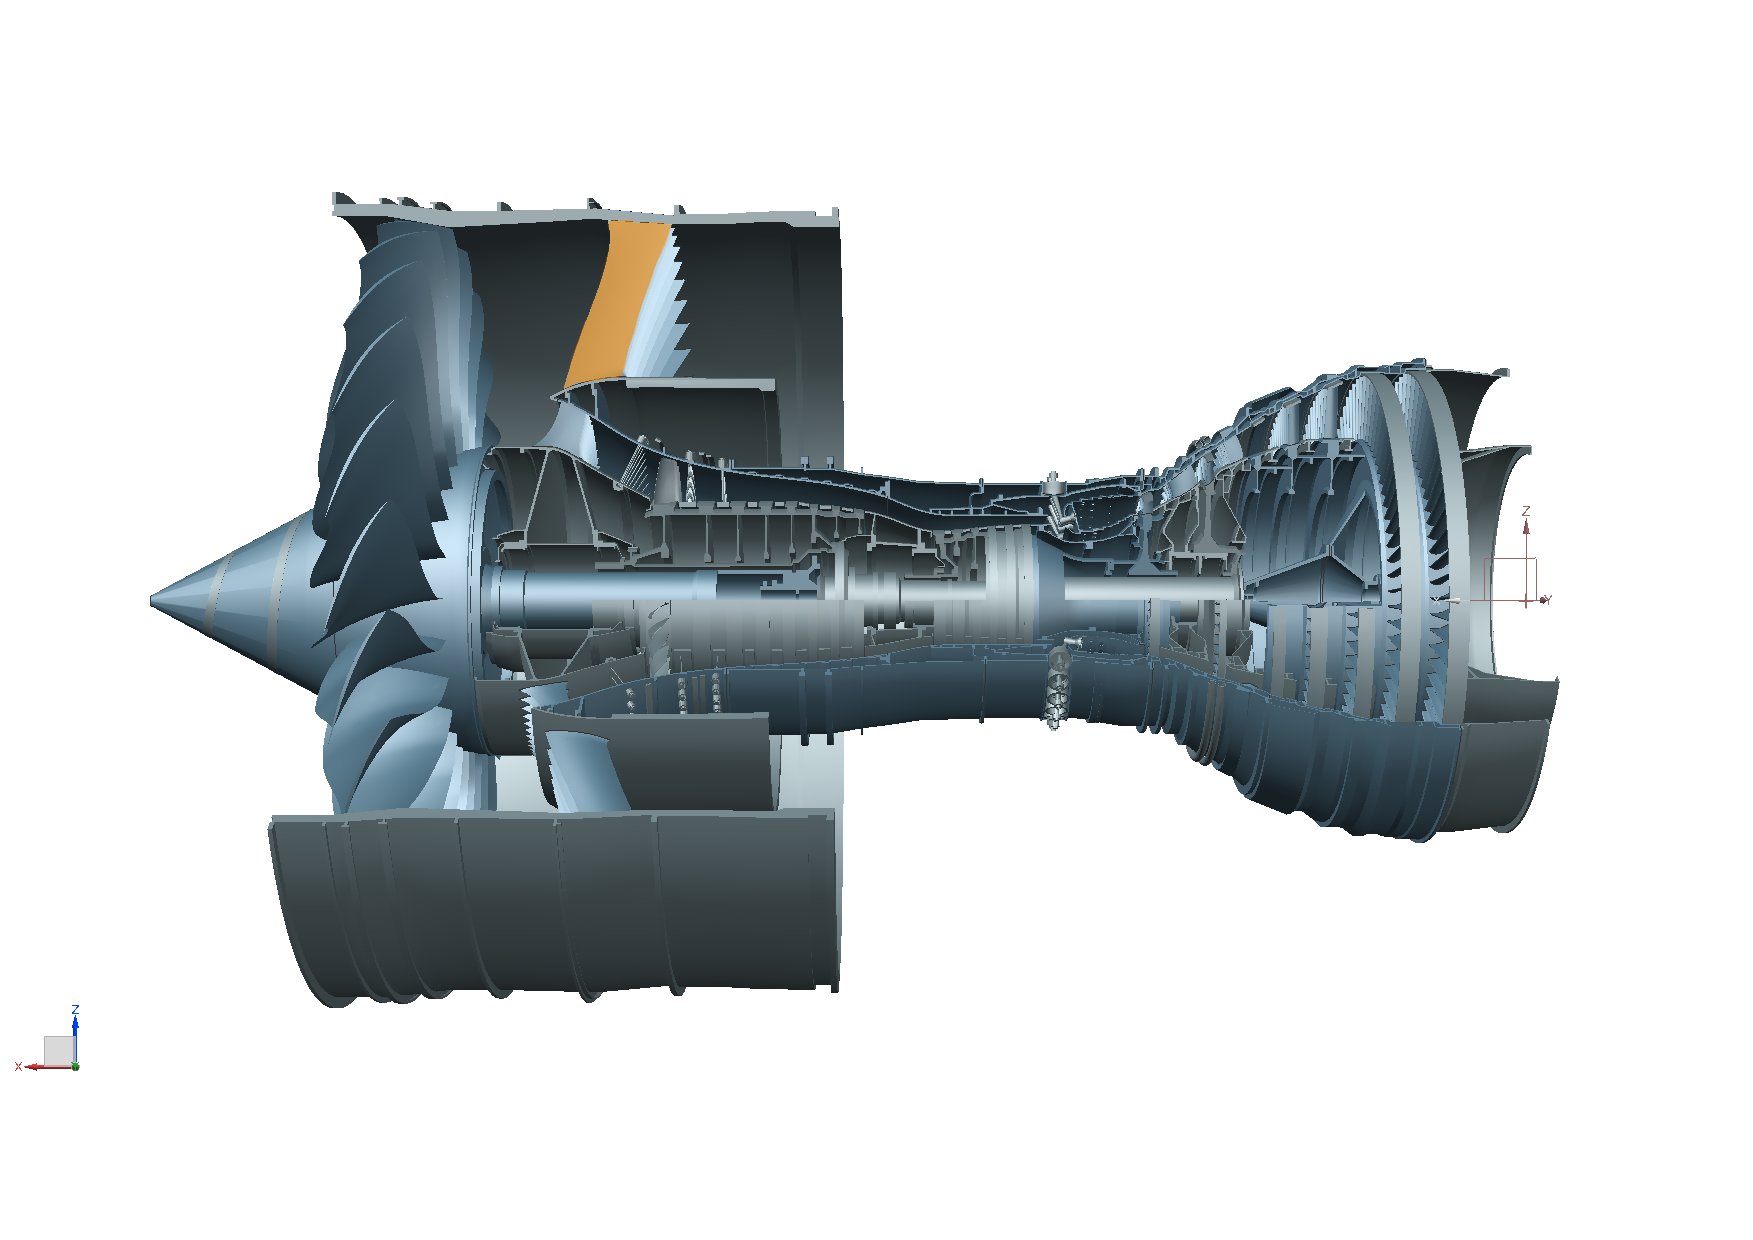
\includegraphics[width=0.9\textwidth]{figures/trent9000_OGV.png}
    \caption{A Rolls Royce Trent 9000 turbine rendered in CAD, with one \ac{FF} \ac{OGV} highlighted in orange.\Jakob{add a render of an OGV as a figure b}}
    \label{fig:my_label}
\end{figure}

\Jakob{present an illustration of the simple sample vane, geometry and EF-M}

\subsection{Novel concepts}

\Jakob{presentation of some of the DS/FR from the july workshop, and implementation in omfgDSE (mechanic turk style)}

\Jakob{
In the workshop, 10 relevant new DS were introduced (compared to legacy design)

2 new functions were introduced
}

% new solutions
The innovation workshop resulted in ten novel alternative design solutions over the legacy design.
Their nature ranged from material alternatives over different interface approaches to variations in shape and dimensions of the existing solutions.
Exemplary for the different new solution, one set of alternative DS is presented here in both the functional and geometrical domain, as well as the respective elements of the \ac{OMFG} linking those two domains.

% new solutions example
The \ac{FR} "Join vane to fitting" is in the legacy design solved by the \ac{DS} "Adhesive connection", meaning that the vane is glued to the fitting using \Jakob{Find right glue name here}.
The workshop results contained the alternative DS "Bolted joint" and "Fully integrated solution", as is shown in Figure \ref{fig:altSolutionEFM}.

Each of the solutions was modelled as an \ac{UDF} in Siemens NX, and the resulting UDF was coupled to the EF-M model through the \ac{OMFG}.
The resulting \textit{UDF} and \textit{interface} objects in the \ac{OMFG}, as well as the geometry, are illustrated in Figure \ref{fig:altSolutionOmfg}.

% instantiated 

\subsection{Method reception}
\Jakob{opinions }

“I enjoyed it; seemed fun; learned a lot of things just by reading the graph” [Aerodynamics analysis engineer]


\section{Discussion}

\section{Conclusions}
\Jakob{
\begin{itemize}
    \item function modelling a good approach
    \item EF-M too strict - e.g. 1:1 solution function modelling unrealistic
    \item CAD Linkage really benefitial, even though hard to code
    \item good first step in DSE approach - generally benefitial for conceptual PD
\end{itemize}
}

\section*{Acknowledgements}

This work was funded in the VINNOVA project MEPHISTO and executed in coopertaion with GKN Aerospace.

\bibliography{references}

\end{document}